\chapter{Life Cycle of Cyclones in the Southwestern Atlantic}

This chapter explores the diverse life cycle configurations, statistical analyses, and geographical distribution of cyclones within the Southwestern Atlantic and South American Southeastern region (SESA). The analysis is conducted using the Cyclophaser program, which facilitates detailed examination of cyclone behaviors and patterns. While part of the results presented here is present in \textbf{CITATION}, here the focus is on the SESA region. In contrast, the cited study encompasses a broader examination, including all cyclogenesis regions across the South Atlantic, extending to the Antarctic Peninsula and the Weddell Sea.


\subsection{Climatological Aspects and Life Cycle Configurations}

Using the tracking methodology described in Section \ref{track_method}, the TRACK algorithm identified 33,376 cyclone systems in the South Atlantic region from 1979 to 2020. The focus here was on systems originating from the SESA region, specifically from SE-BR, LA-PLATA, and ARG genesis regions. After filtering to include only these tracks, the number of systems was narrowed down to 7,931 (Figure \ref{fig:pie_climatology}). Among these, 56\% originated in the ARG region, 23.6\% in LA-PLATA, and 20.4\% in SE-BR. This distribution and general seasonality aligns with previous studies by \citet{gramcianinov2019properties} and \citet{crespo2021potential}. However, the SE-BR region exhibited a higher relative frequency in this analysis, potentially attributable to the finer resolution of the ERA5 dataset used here compared to previous studies \citep{gramcianinov2020analysis}. However, comparing the seasonal distribution with earlier studies introduces complexities due to variations in the definitions and boundaries of genesis regions \citep[e.g.,]{reboita2010regimes, crespo2021potential}.

\begin{figure}[ht]
    \centering
    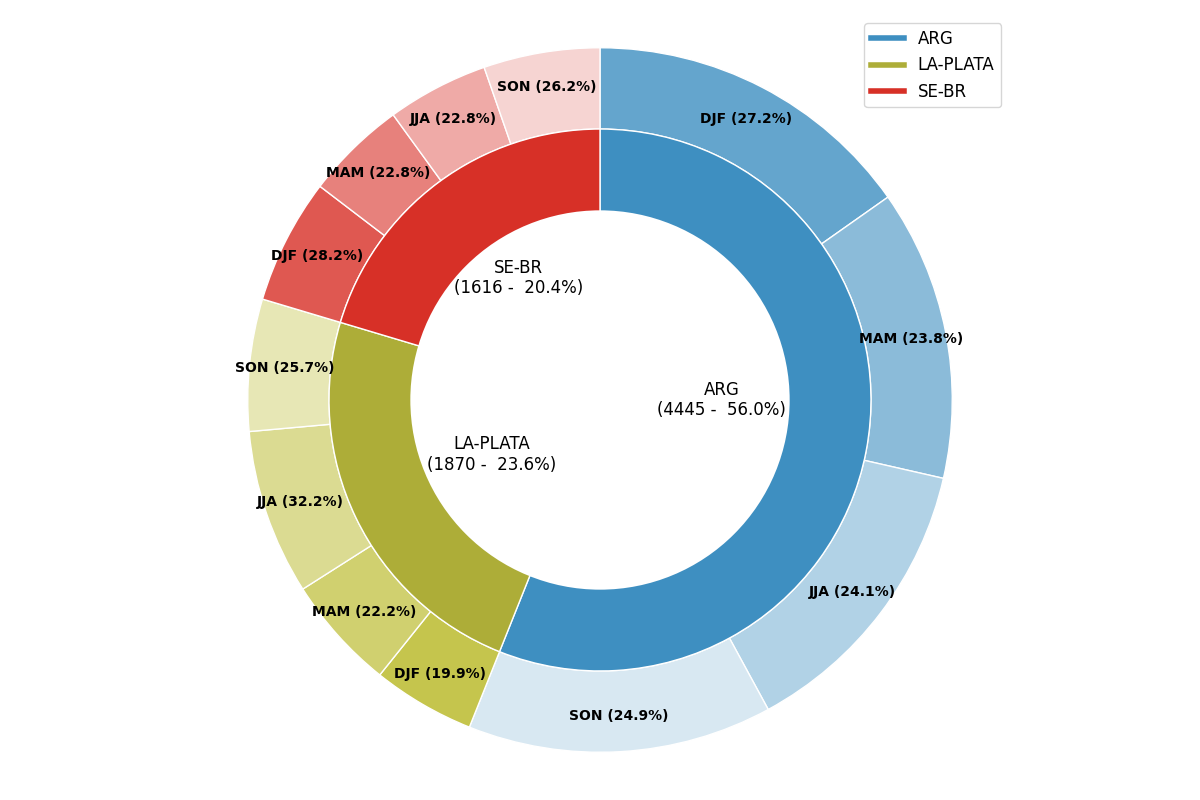
\includegraphics[width=\textwidth]{figs_4/pie_systems_count.png}
    \caption[Cyclogenesis Climatology in the SESA Region]{Number of systems and their relative frequencies by genesis region in the SESA region for the period 1979-2020. The inner pie chart displays the total frequency of systems by region, while the outer ring shows the seasonal distribution of cyclogenesis within each region.}
\label{fig:pie_climatology}
\end{figure}


During the period from 1979 to 2020, cyclonic systems originating from the ARG, LA-PLATA, and SE-BR regions demonstrated 41 distinct life cycle configurations (Figure \ref{fig:all_lifecycle_configurations}). Most configurations did not account for more than 1\% of the total system count, typically lacking a mature stage. This phenomenon is likely due to these systems having maturation stages shorter than the CycloPhaser's threshold for detecting this phase. Adjusting the threshold to recognize shorter mature stages would risk identifying spurious cycles.


\begin{figure}[ht]
    \centering
    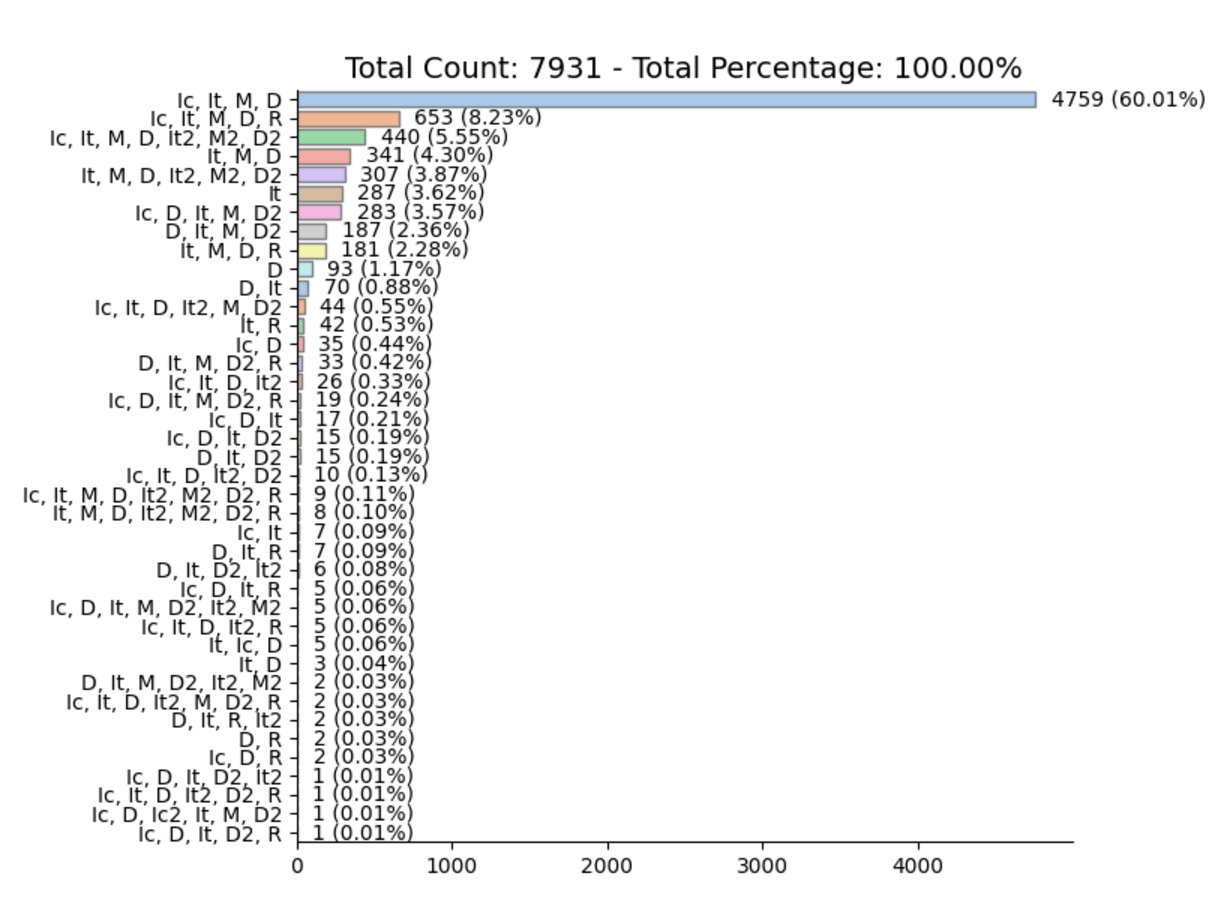
\includegraphics[width=\textwidth]{figs_4/combined_barplots_total_all_systems.pdf}
    \caption[Life cycle configurations]{Distribution of all identified cyclone lifecycle configurations in the SESA region, spanning from 1979 to 2020. The configurations are sorted by their total count (frequency), with each bar representing the total number of cyclones exhibiting a specific lifecycle pattern, containing distinct stages: incipient (Ic), intensification (It), mature (M), decay (D), and residual (R), showing their sequence within the lifecycle.}
\label{fig:all_lifecycle_configurations}
\end{figure}

To focus on significant life cycle patterns, it was filtered the configurations to include only those comprising at least 1\% of all types (Figure \ref{fig:filtered_lifecycle_configurations}). This criterion reduced the sample size to 7,531 systems, accounting for approximately 95\% of the original database. It was also merged life cycle counts that differed solely by the inclusion of a residual stage, as these are not indicative of the system's actual development (as discussed in Section \ref{sec:cyclophaser_description}). Further, to avoid bias in phase statistics, it was excluded life cycles lacking a mature phase. For instance, systems exhibiting only intensification and/or decay phases might have longer durations for these phases compared to others, potentially skewing statistics. Such configurations might represent undeveloped systems exiting the tracking domain before maturation. With these filters applied, the number of systems analyzed was reduced to 7,151, representing about 90\% of the initial count of systems with genesis in the SESA region (Figure \ref{fig:filtered_lifecycle_configurations}b).

\begin{figure}[ht]
\centering
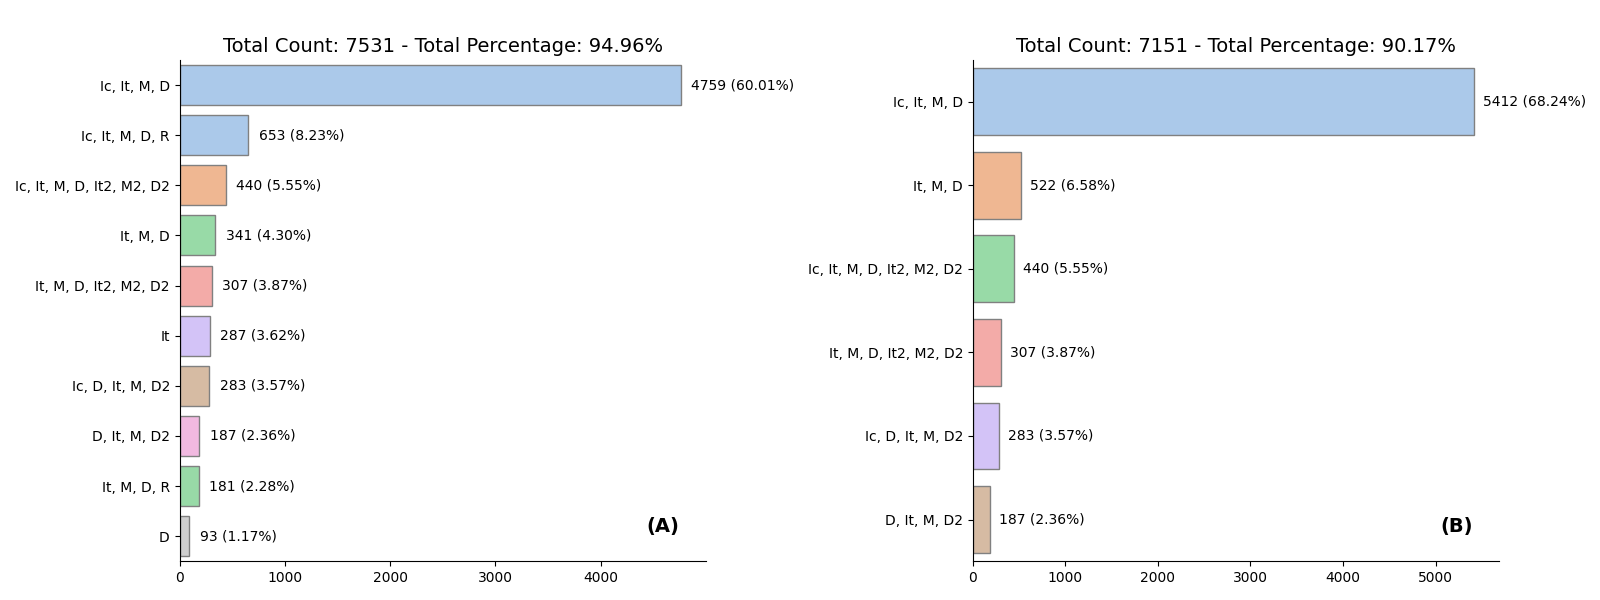
\includegraphics[width=\textwidth]{figs_4/combined_barplots_filtered.png}
\caption[Filtered life cycle configurations]{(a) Lifecycle configurations of cyclones that represent at least 1\% of the total identified patterns. (b) Adjusted lifecycle configurations after merging periods classified as residual and removing stages not contributing to a standard development pattern, focusing analysis on the core developmental stages of cyclones.}
\label{fig:filtered_lifecycle_configurations}
\end{figure}

Figure \ref{fig:representative_life_cycles} depicts representative cases for each life cycle configuration retained for analysis (as shown in Figure \ref{fig:filtered_lifecycle_configurations}b). The most common configuration in the SESA region typically follows the expected development pattern of extratropical cyclones: incipient, intensification, mature, and decay stages (Figure \ref{fig:representative_life_cycles}a), accounting for 68\% of all evaluated systems. The second most common type mirrors this sequence but omits the incipient stage, indicating a rapid intensification process (Figure \ref{fig:representative_life_cycles}b). The third and fourth most frequent types depict a repeated complete cycle, including a secondary intensification, mature, and decay phases, with the third type including an incipient stage (Figure \ref{fig:representative_life_cycles}c) and the fourth lacking one (Figure \ref{fig:representative_life_cycles}d). The fifth and sixth configurations exhibit an early decay stage, differentiated by the presence (Figure \ref{fig:representative_life_cycles}e) or absence (Figure \ref{fig:representative_life_cycles}f) of an incipient phase.

\begin{figure}[h!]
\centering
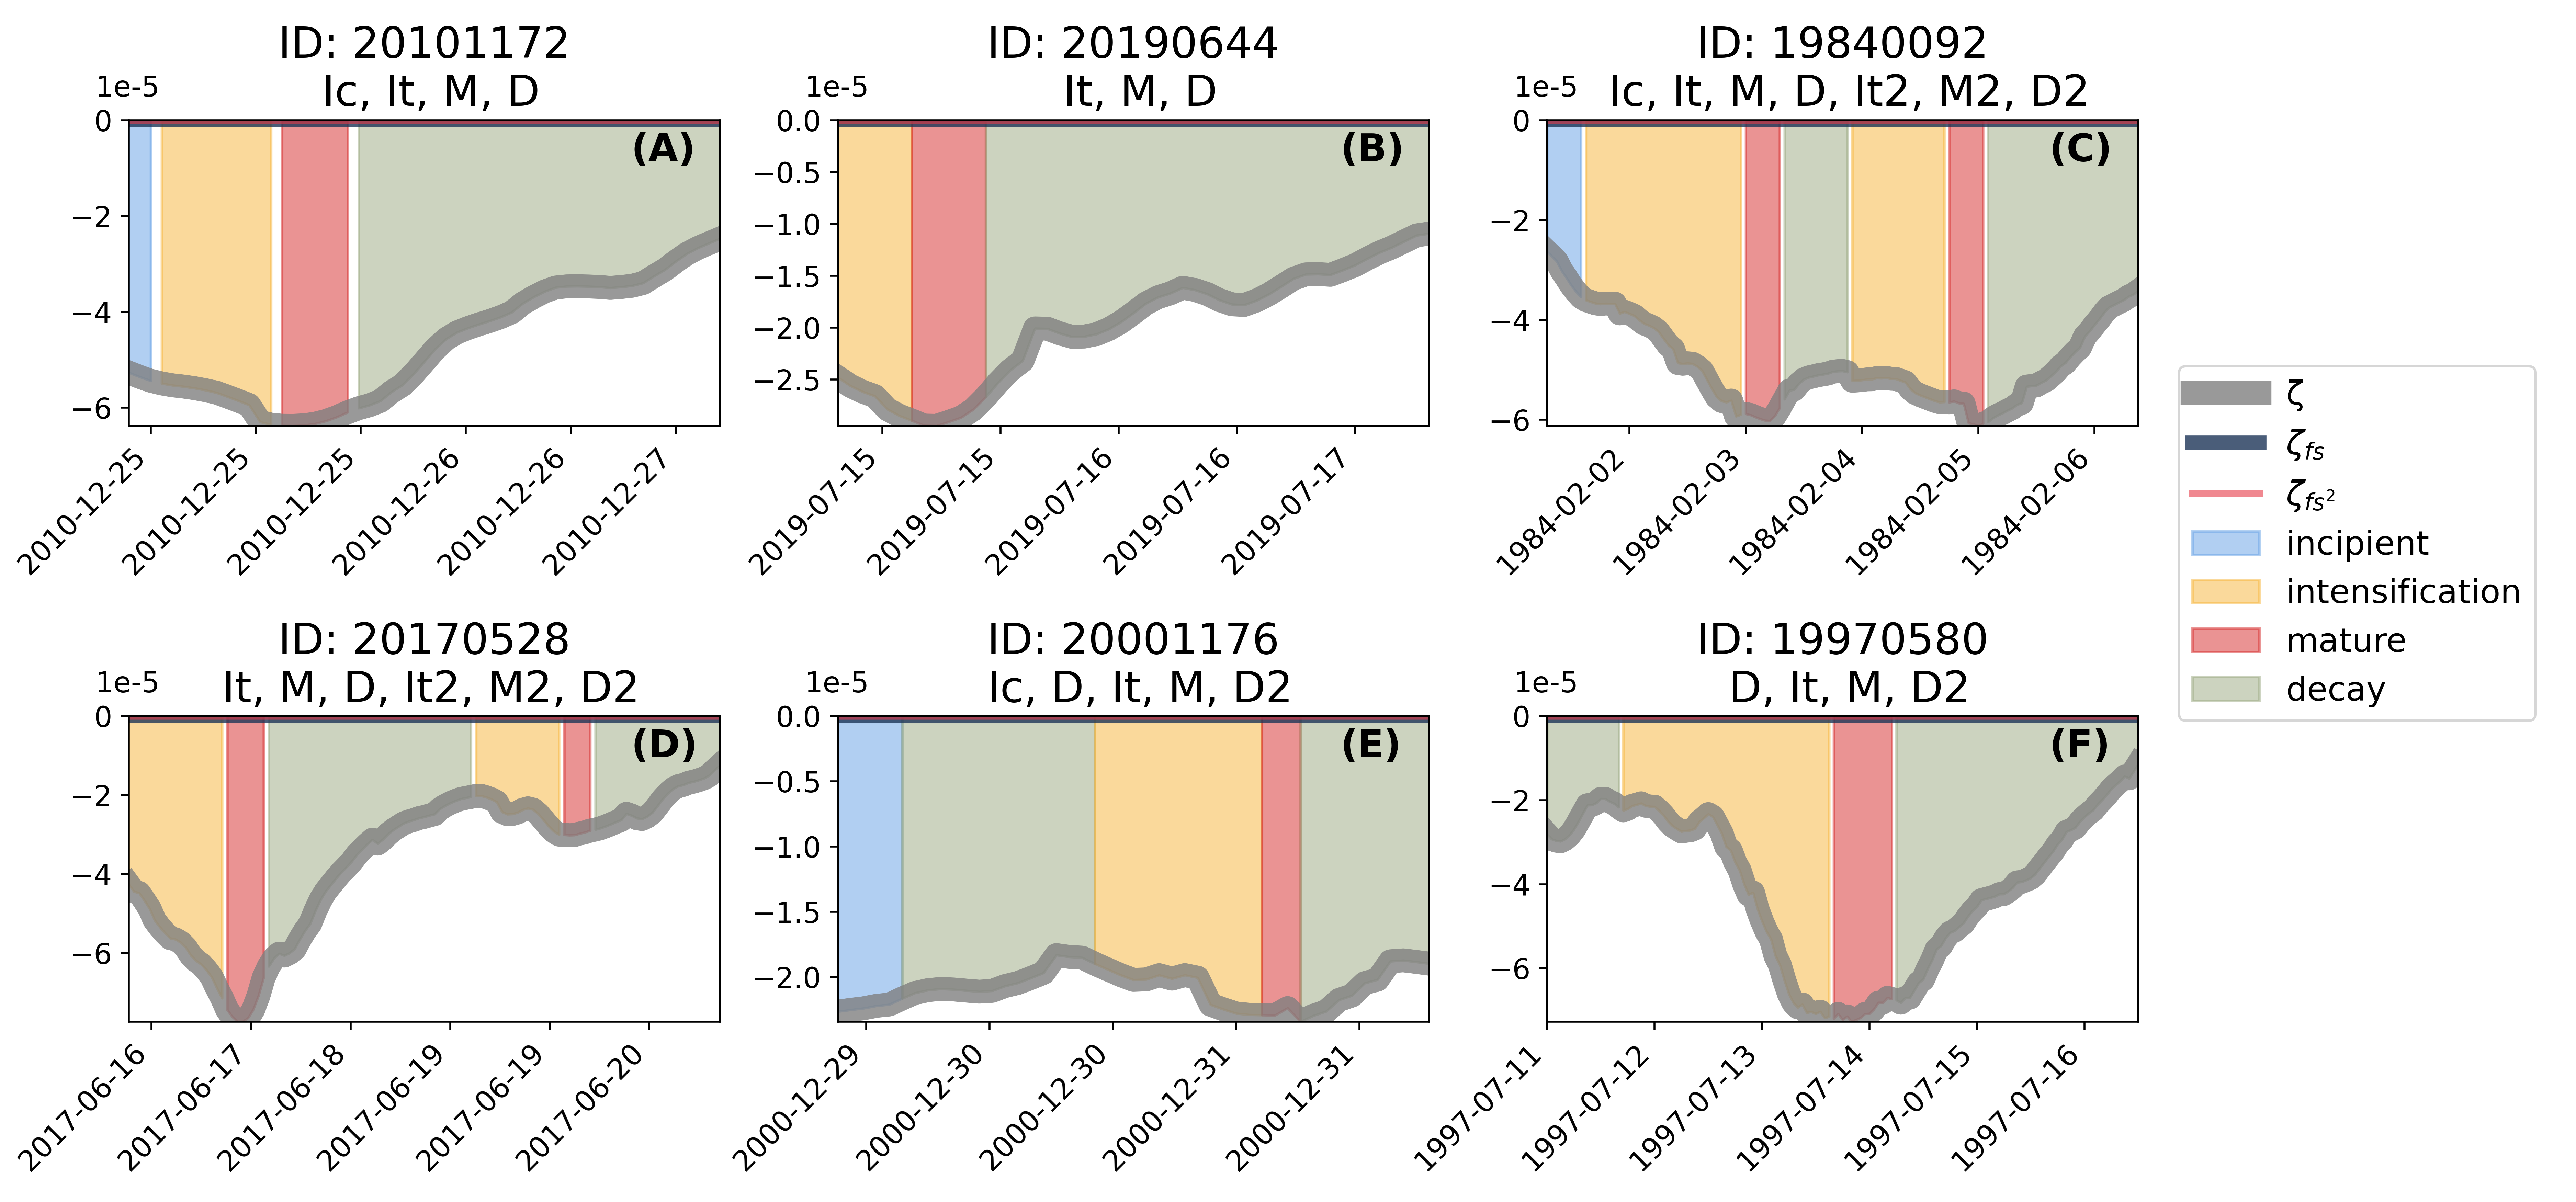
\includegraphics[width=\textwidth]{figs_4/main_species_life-cycle.png}
\caption{Representative examples of cyclone life cycles for configurations shown in Figure \ref{fig:filtered_lifecycle_configurations}b. Panels A to F illustrate the central relative vorticity \(\zeta_{850}\) and its first (\(\zeta_{fs}\)) and second (\(\zeta_{fs^2}\)) smoothed derivatives. Background colors indicate different life cycle phases: : incipient (Ic), intensification (It), mature (M) and decay (D). Lines represent the original vorticity series (\(\zeta\)), the first (\(\zeta_{fs}\)), and the second (\(\zeta_{fs^2}\)) smoothed relative vorticity series.}
\label{fig:representative_life_cycles}
\end{figure}

The analysis reveals minimal to negligible seasonal variability in the frequency of each life cycle configuration across different genesis regions (Figure \ref{fig:lifecycle_configurations_seasonal_variability}). The configurations "Ic, It, M, D" and "Ic, It, M, D, It2, M2, D2" are consistently more frequent, jointly accounting for 60\% to 68\% of all cases across all regions. However, exceptions include the "It, M, D" configuration emerging as the second most frequent in ARG during JJA, and in SE-BR during MAM and JJA. Additionally, the "Ic, D, M, D2" configuration appears significantly more often in LA-PLATA during JJA and in SE-BR during SON.


\begin{figure}[h!]
\centering
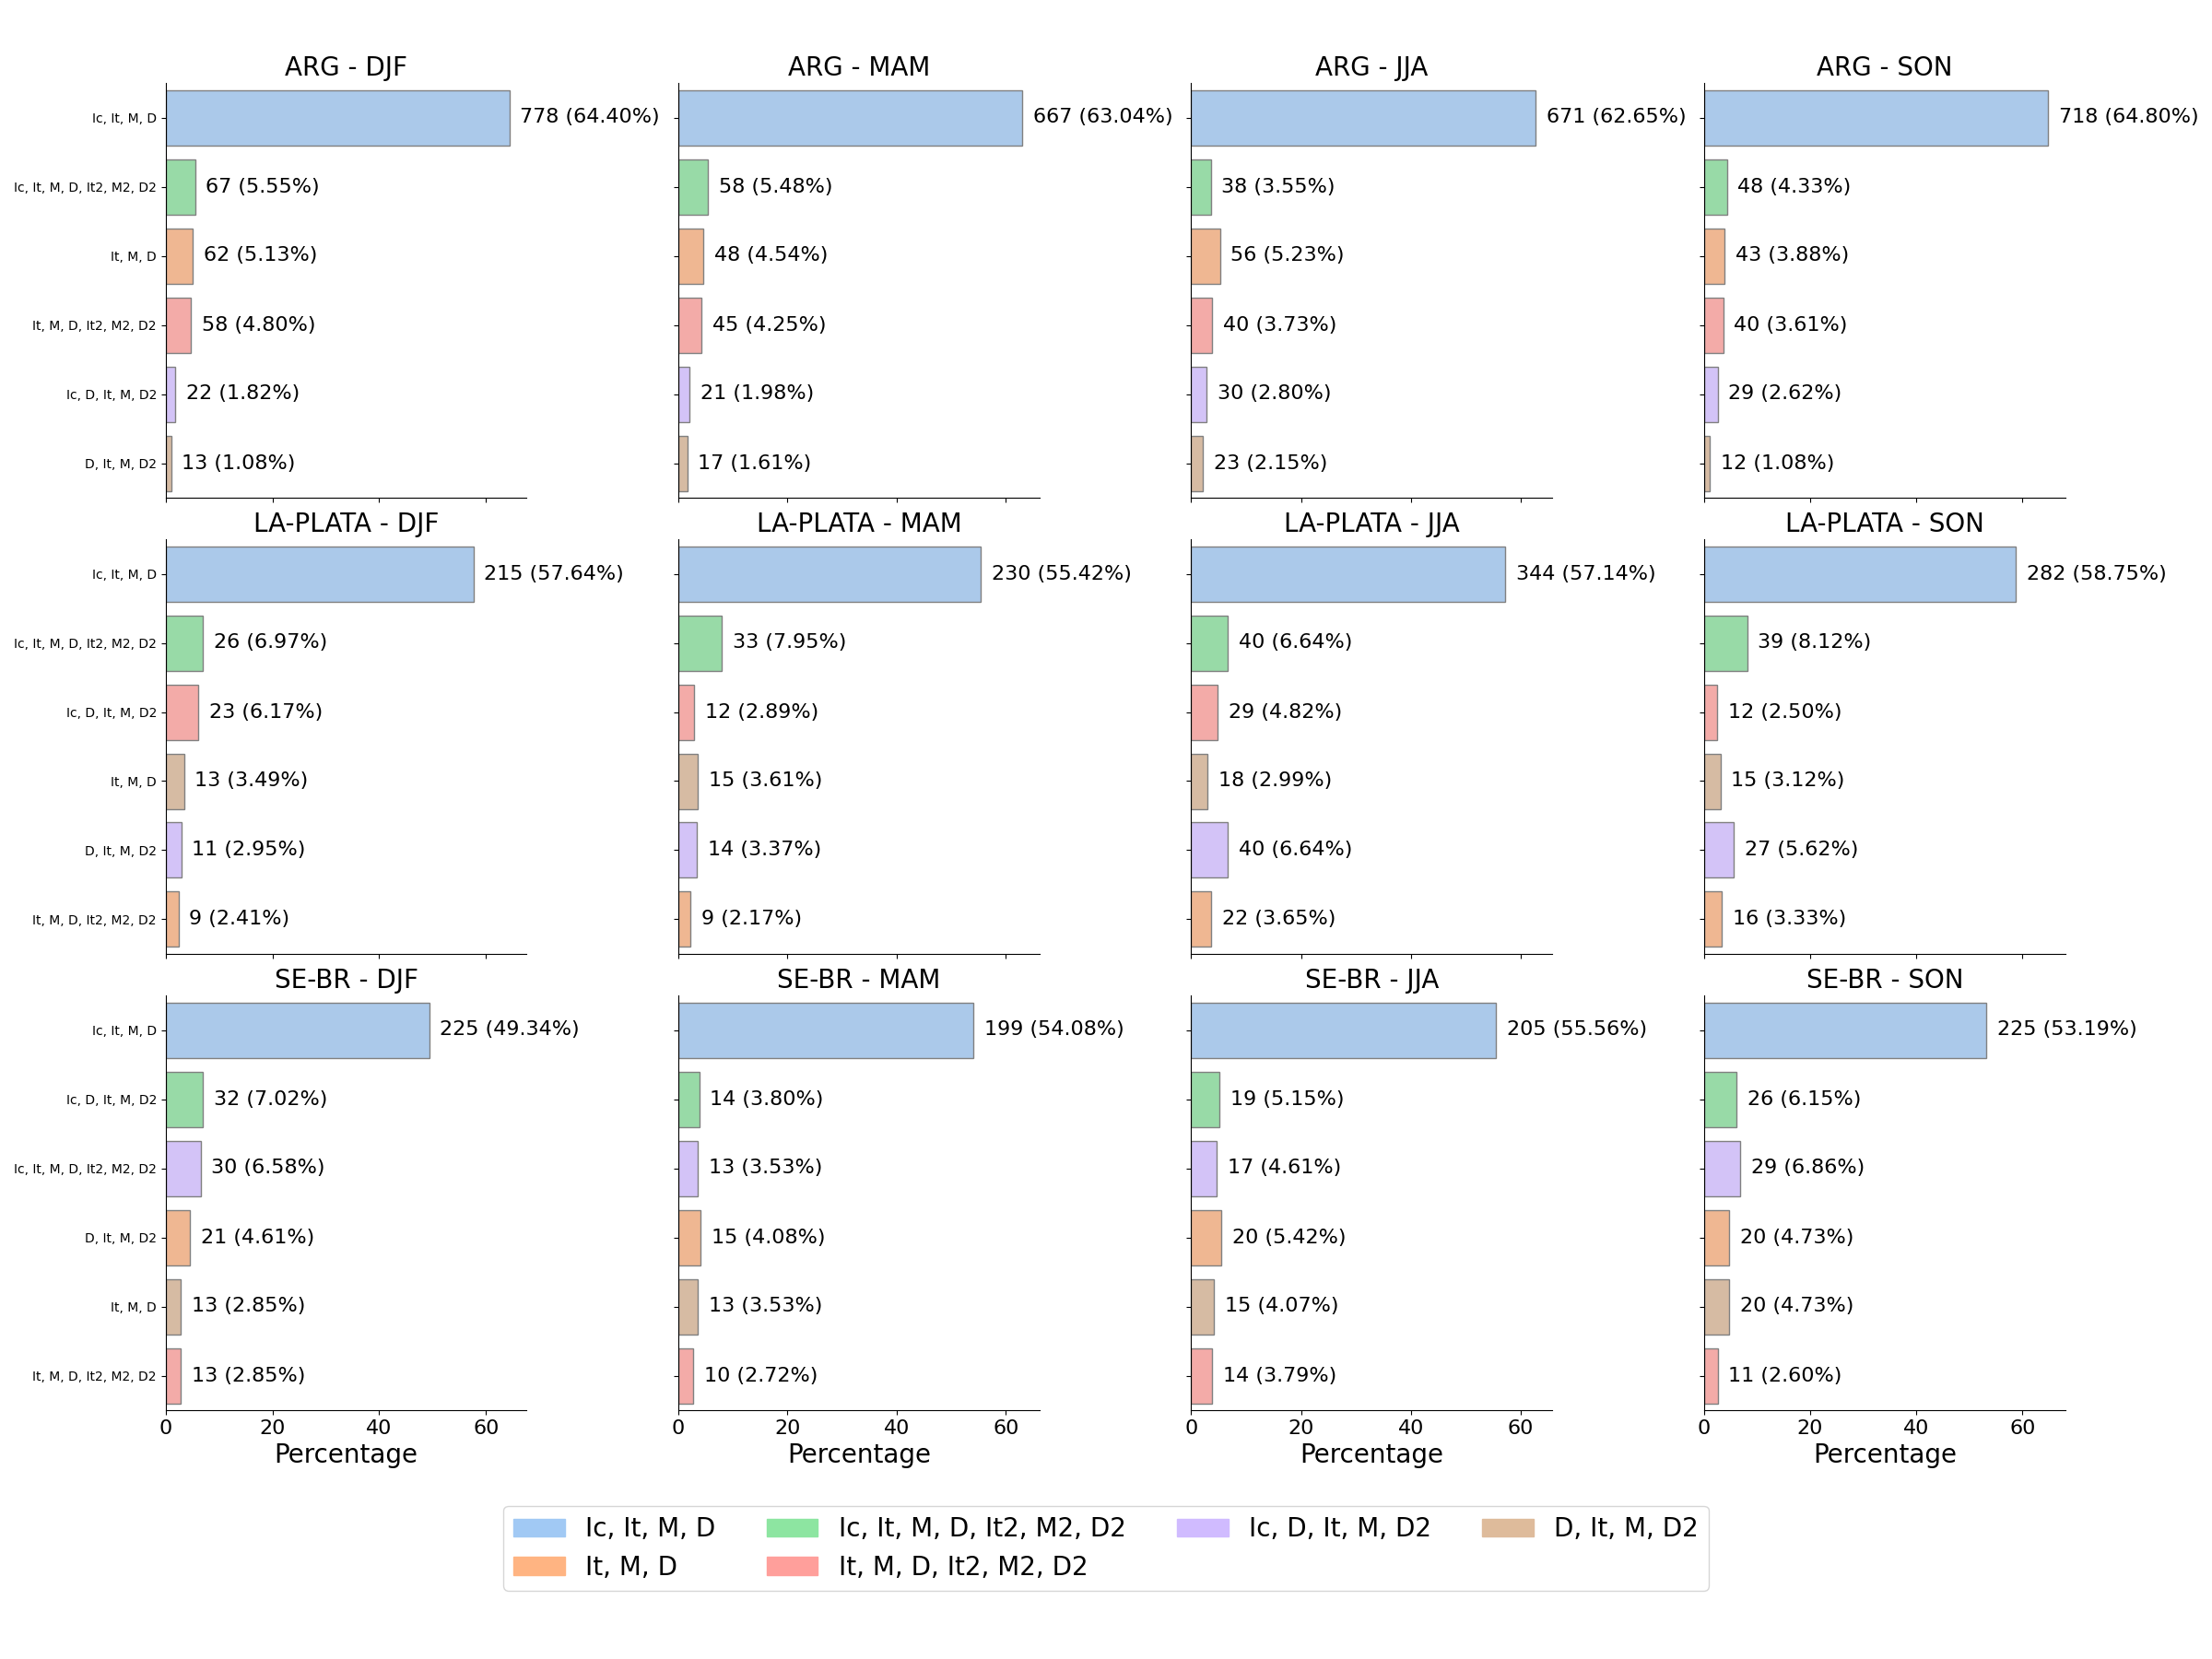
\includegraphics[width=\textwidth]{figs_4/multi_panel_barplots_filtered.png}
\caption[Life cycle configurations by regions and season]{Similar to Figure \ref{fig:filtered_lifecycle_configurations}, but separated by genesis region (ARG, LA-PLATA and SE-BR) and season.}
\label{fig:lifecycle_configurations_seasonal_variability}
\end{figure}


\subsection{Cyclone Statistics}
\label{sec:cyclone_statistics}

This section explores the statistical analysis of cyclones in the SESA region, comparing the constrained data utilized in this study with extant literature. Results are presented both for an aggregate view across all genesis regions and individually by region. To capture the seasonal variability of cyclone behavior, analysis is focused on the winter (JJA) and summer (DJF) months. This approach is chosen because the transitional seasons (MAM and SON) generally display characteristics that are intermediate to those observed in JJA and DJF, aligning with findings from previous climatologies of the SESA region \citep[e.g.]{gan1991surface, reboita2010south, crespo2021potential}. 

On average, cyclones exhibit longer lifespans during DJF, with a duration of $97.6 \pm 66.2$ hours (Figure \ref{fig:pdf_total_time_total}a) compared to $91.1 \pm 59.7$ hours during JJA (Figure \ref{fig:pdf_total_time_total}b). Conversely, the average total distance traveled by cyclones is slightly greater during JJA, amounting to $4777 \pm 3182$ km (Figure \ref{fig:pdf_total_time_total}d), versus $4658 \pm 3212$ km in DJF (Figure \ref{fig:pdf_total_time_total}c). This is reflected in the mean propagation speed, which is higher in JJA at $15.3 \pm 4.8$ m/s (Figure \ref{fig:pdf_total_time_total}f) compared to DJF at $14.0 \pm 4.4$ m/s (Figure \ref{fig:pdf_total_time_total}e).

\begin{figure}[h!]
\centering
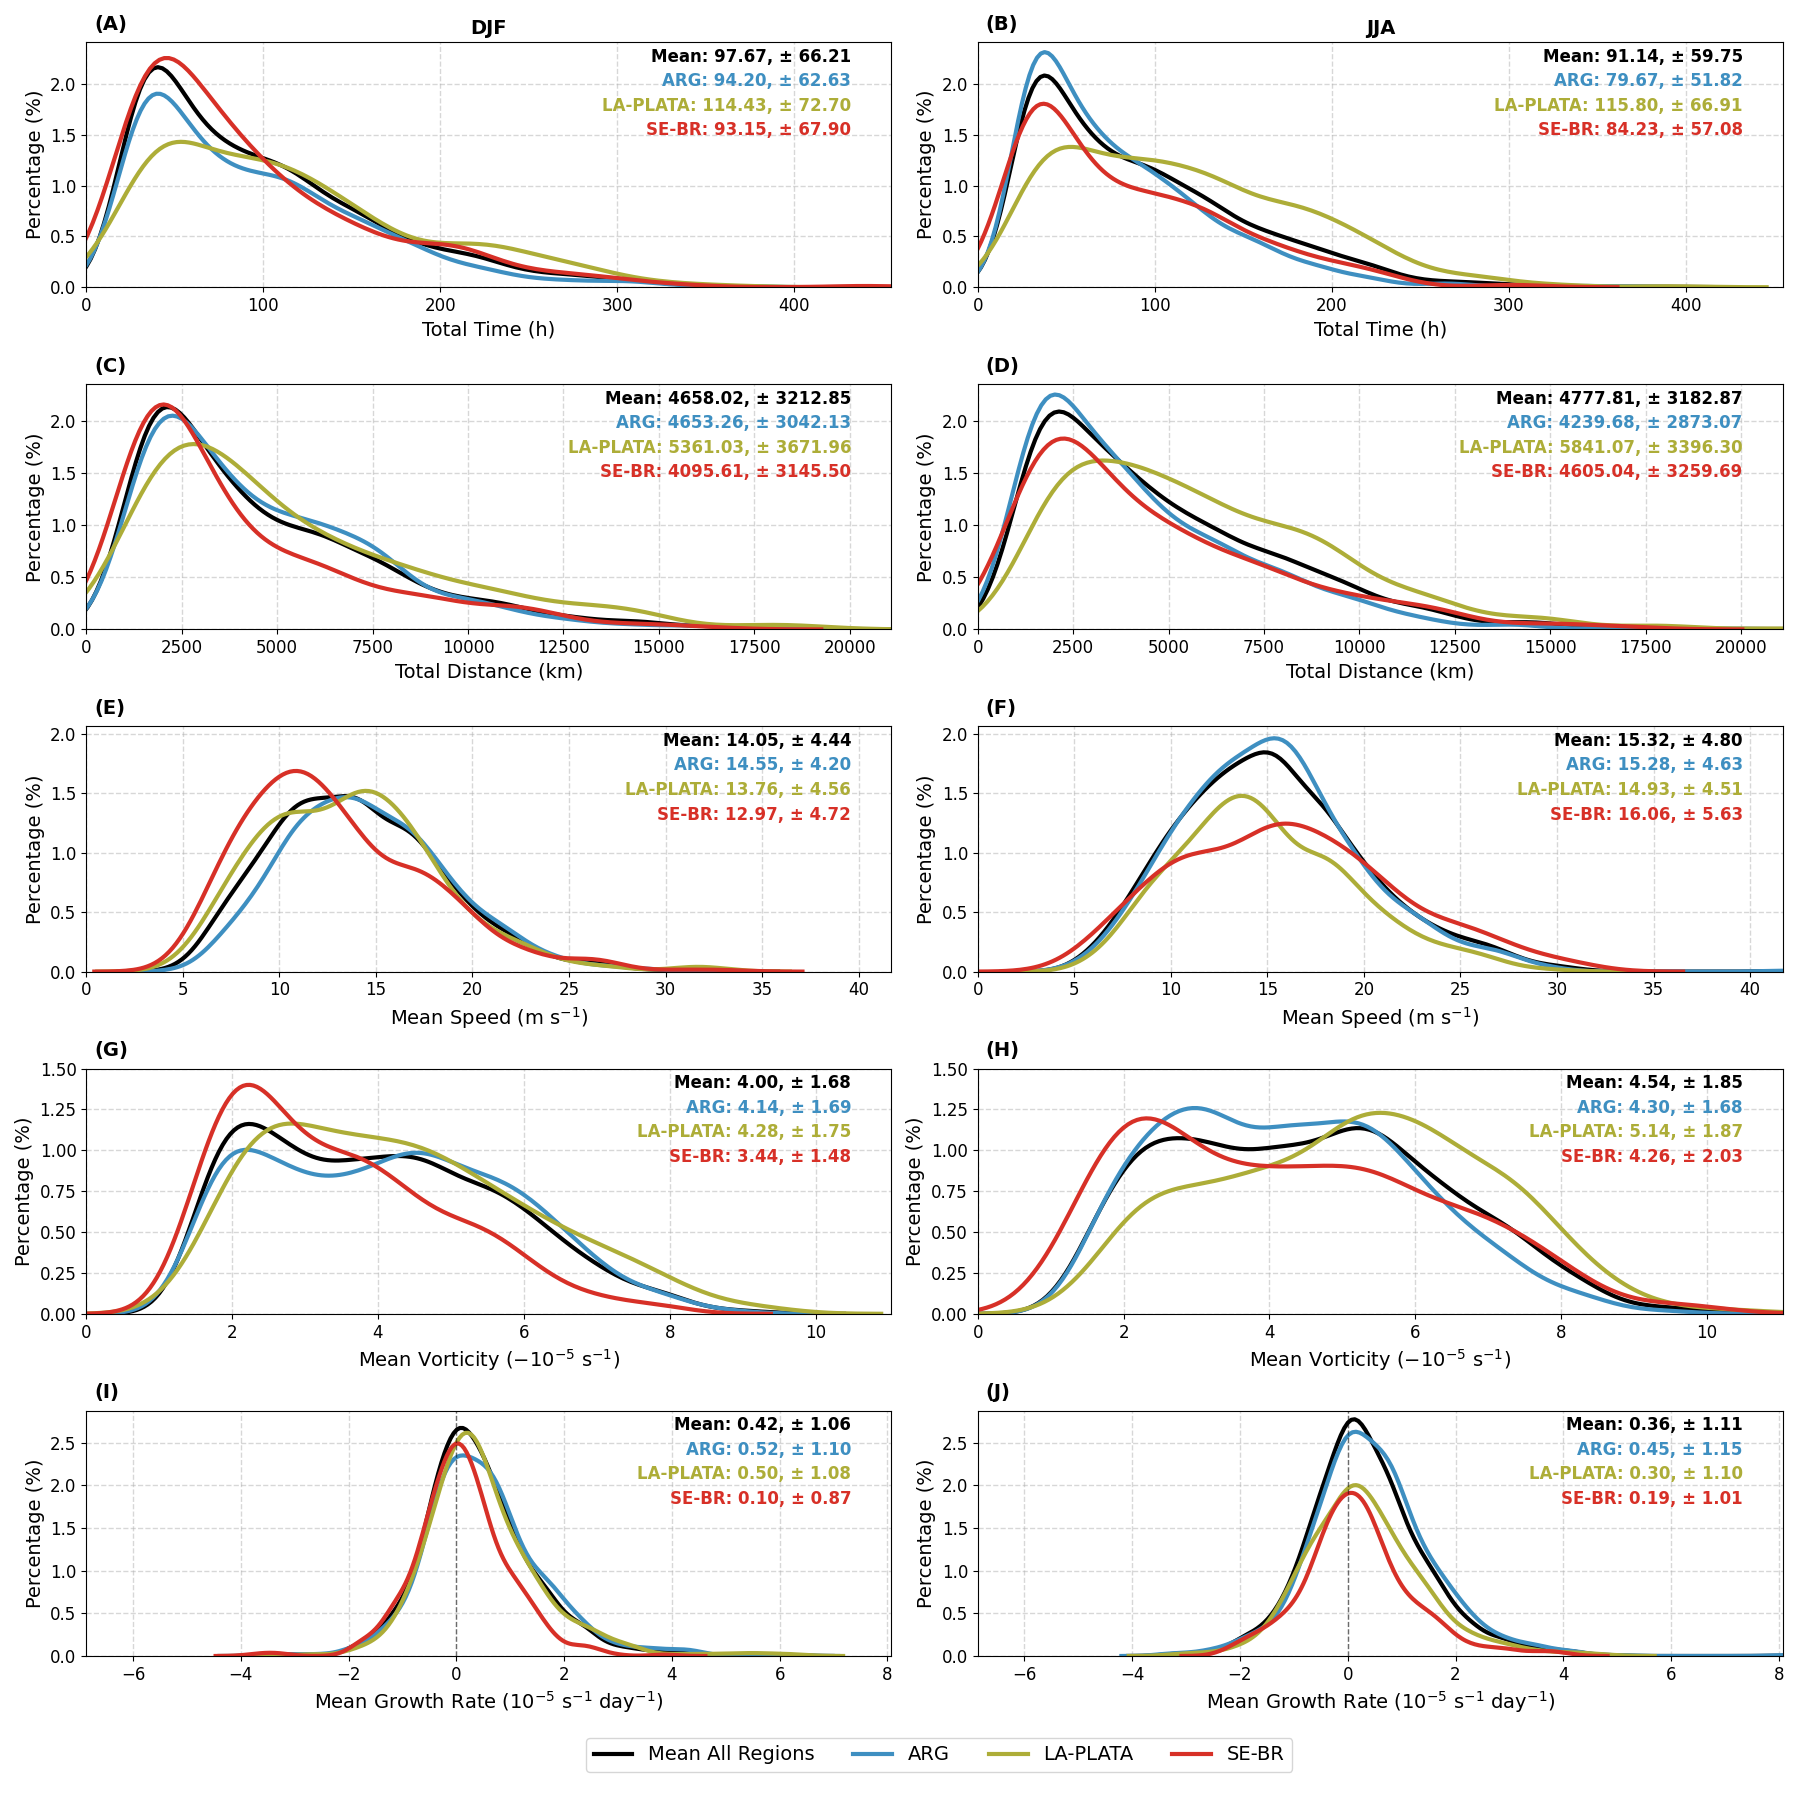
\includegraphics[width=\textwidth]{figs_4/pdf_total_phase_all_metrics.png}
\caption[PDF - Metrics for each region and season]{Probability density functions (PDF) comparing cyclone lifecycle metrics across different genesis regions (ARG, LA-PLATA, SE-BR) for DJF and JJA. Each panel displays the density distributions for a specific metric: total time (A and B), total distance (C and D), mean speed (E and F), mean vorticity (G and H), and mean growth rate (I and J). The lines in each graph represent the mean values for all regions combined (black), ARG (blue), LA-PLATA (green), and SE-BR (red), while the annotations represent the mean and standard deviation values.}
\label{fig:pdf_total_time_total}
\end{figure}

These results largely corroborate those by \citet{gramcianinov2019properties, gramcianinov2020analysis, hoskins2005new} and exceed the mean duration, traveled distance, and propagation speed reported by \citet{simmonds2000mean}, \citet{mendes2010climatology}, and \citet{reboita2010south}. The disparities likely stem from differing tracking methodologies, data sets, and the exclusion of systems without a mature phase in our analysis. Particularly, the exclusion of continental systems may inflate displacement statistics during austral summer when quasi-stationary lows are prevalent over the continent \citep{mendes2010climatology}. Furthermore, \citet{reboita2010south} focused on oceanic systems, which might have overlooked early development stages, and their use of relative vorticity at 10m, impacted by surface drag, could account for variations in propagation speed.

The analysis reveals notable inter-regional variability in cyclone behavior, with trends predominantly mirroring those observed in the ARG region, which accounts for the highest frequency of cyclone occurrences within the SESA region (Figure \ref{fig:pie_climatology}). When examining total cyclone duration, distinct seasonal patterns emerge: both the ARG and SE-BR regions exhibit significantly shorter lifespans during JJA compared to DJF, with the probability density functions (PDFs) peaking at approximately 50 hours. In contrast, the LA-PLATA region shows slightly longer durations during JJA, with a mean difference of about 1.5 hours. Additionally, the distribution of cyclone durations in the LA-PLATA region is more right-skewed than in ARG and SE-BR, indicating greater variability in the lifespan of cyclones originating from LA-PLATA. Across all regions, the standard deviation decreases from DJF to JJA, suggesting a higher occurrence of longer-lasting cyclones during the summer months.

In terms of displacement, the ARG region displays shorter average distances during DJF compared to JJA, whereas LA-PLATA and SE-BR exhibit increases, particularly notable in SE-BR. Similar to the trends in duration, the displacement patterns in ARG and SE-BR exhibit distinct peaks at approximately 2500 km, while LA-PLATA shows a more right-skewed distribution, especially during JJA, indicating greater variability in cyclone travel distances. These regional differences in displacement are also mirrored in the average propagation speeds of the cyclones: during DJF, cyclones in ARG generally move faster than those in LA-PLATA and SE-BR. This changes in JJA, with SE-BR exhibiting the highest increases in speed, making it the region with the most mobile cyclones during this season, followed by ARG and then LA-PLATA. This variation is reflected in the PDFs for each region: during DJF, SE-BR's propagation speed peaks at approximately \(10 \, \text{m s}^{-1}\) and ARG at \(13 \, \text{m s}^{-1}\), while LA-PLATA displays a bimodal distribution with peaks at approximately \(10 \, \text{m s}^{-1}\) and \(15 \, \text{m s}^{-1}\). During JJA, the peak for ARG shifts to approximately \(16 \, \text{m s}^{-1}\), and LA-PLATA's distribution changes to peak at around \(14 \, \text{m s}^{-1}\), while SE-BR assumes a bimodal shape, peaking at roughly \(10 \, \text{m s}^{-1}\) and \(16 \, \text{m s}^{-1}\).

The PDFs for the mean vorticity values of the examined systems display a bimodal, right-skewed distribution with peaks near \(2 \times 10^{-5} \, \text{s}^{-1}\) and \(4 \times 10^{-5} \, \text{s}^{-1}\), with a higher occurrence percentage near the first peak and an average value of \(4 \pm 1.68 \times 10^{-5} \, \text{s}^{-1}\) during DJF (Figure \ref{fig:pdf_total_time_total}g). In JJA, the peaks are positioned near \(2 \times 10^{-5} \, \text{s}^{-1}\) and \(5 \times 10^{-5} \, \text{s}^{-1}\), but with a higher occurrence percentage at the second peak, reflecting an overall increase in mean vorticity, especially in the LA-PLATA region (Figure \ref{fig:pdf_total_time_total}h). The ARG region presents a PDF mirroring the mean cyclone behavior, and SE-BR peaks near \(2 \times 10^{-5} \, \text{s}^{-1}\) in both seasons, being more right-skewed in JJA, which reflects the occurrence of weaker systems in this region. Meanwhile, LA-PLATA shifts from being right-skewed in DJF to left-skewed in JJA, reflecting a significant increase in the intensity of systems in this region. These results highlight the previous findings that LA-PLATA presents the most intense systems in the SESA regions, while SE-BR, the weakest \citep{simmonds2000mean, reboita2010south, gramcianinov2019properties}. Although the regional and seasonal variability largely corroborates findings from \citet{gramcianinov2019properties}, the intensity of cyclones reported here is somewhat smaller, possibly due to the ERA5 dataset be able to detect less intense systems \citep{gramcianinov2020analysis}.

The mean growth rate distribution, is symmetric around zero with a low standard deviation, indicating a dynamic equilibrium in system intensity throughout the life cycle, marked by neither consistent intensification nor weakening, which will be later discussed for each individual phase. It is important to note that these values were computed from normalized relative vorticity data, where positive values suggest system intensification (\(\zeta_{850}\) increasing in magnitude), while negative values indicate a decay (\(\zeta_{850}\) decreasing in magnitude). Overall, although the differences are minimal, the results suggest slightly more intense intensification during DJF (Figure \ref{fig:pdf_total_time_total}i) compared to JJA (Figure \ref{fig:pdf_total_time_total}j), with the latter exhibiting higher mean values.

\subsection{Life Cycle Phase Statistics}
\label{sec:life_cycle_phase_statistics}

This section examines the statistical characteristics of cyclones, exploring various metrics describing cyclonic behavior throughout distinct lifecycle phases. This unique approach is enabled by the Cyclophaser program, offering a more granular analysis than previously available in the literature. As shown in Section \ref{sec:cyclone_statistics}, the region mean results predominantly reflect the ARG region's behavior and hence, region-specific results are detailed here.

Figure \ref{fig:pdf_total_time} displays the PDFs for the mean total time spent in each development phase. These PDFs are right-skewed, indicating high variability across different phases but smaller seasonal and regional differences. Typically, the incipient, mature, and second mature phases show the shortest average durations, often peaking between 3 and 5 hours. The intensification, second intensification, and decay phases often exhibit longer tails, suggesting a wide variability in their durations. In the ARG region, all phases show a slight reduction in mean duration from DJF (Figure \ref{fig:pdf_total_time}a) to JJA (Figure \ref{fig:pdf_total_time}b), with decay and second decay stages exhibiting the most significant reductions, indicating that shorter average total durations in JJA are primarily due to these phases (Figure \ref{fig:pdf_total_time_total}). For LA-PLATA and SE-BR, notable changes include particularly variations in the standard deviations of the second intensification and decay phases, and in the decay phase for SE-BR, suggesting that seasonal differences in total mean durations for these regions are largely attributable to fluctuations in extreme values.

\begin{figure}[h!]
\centering
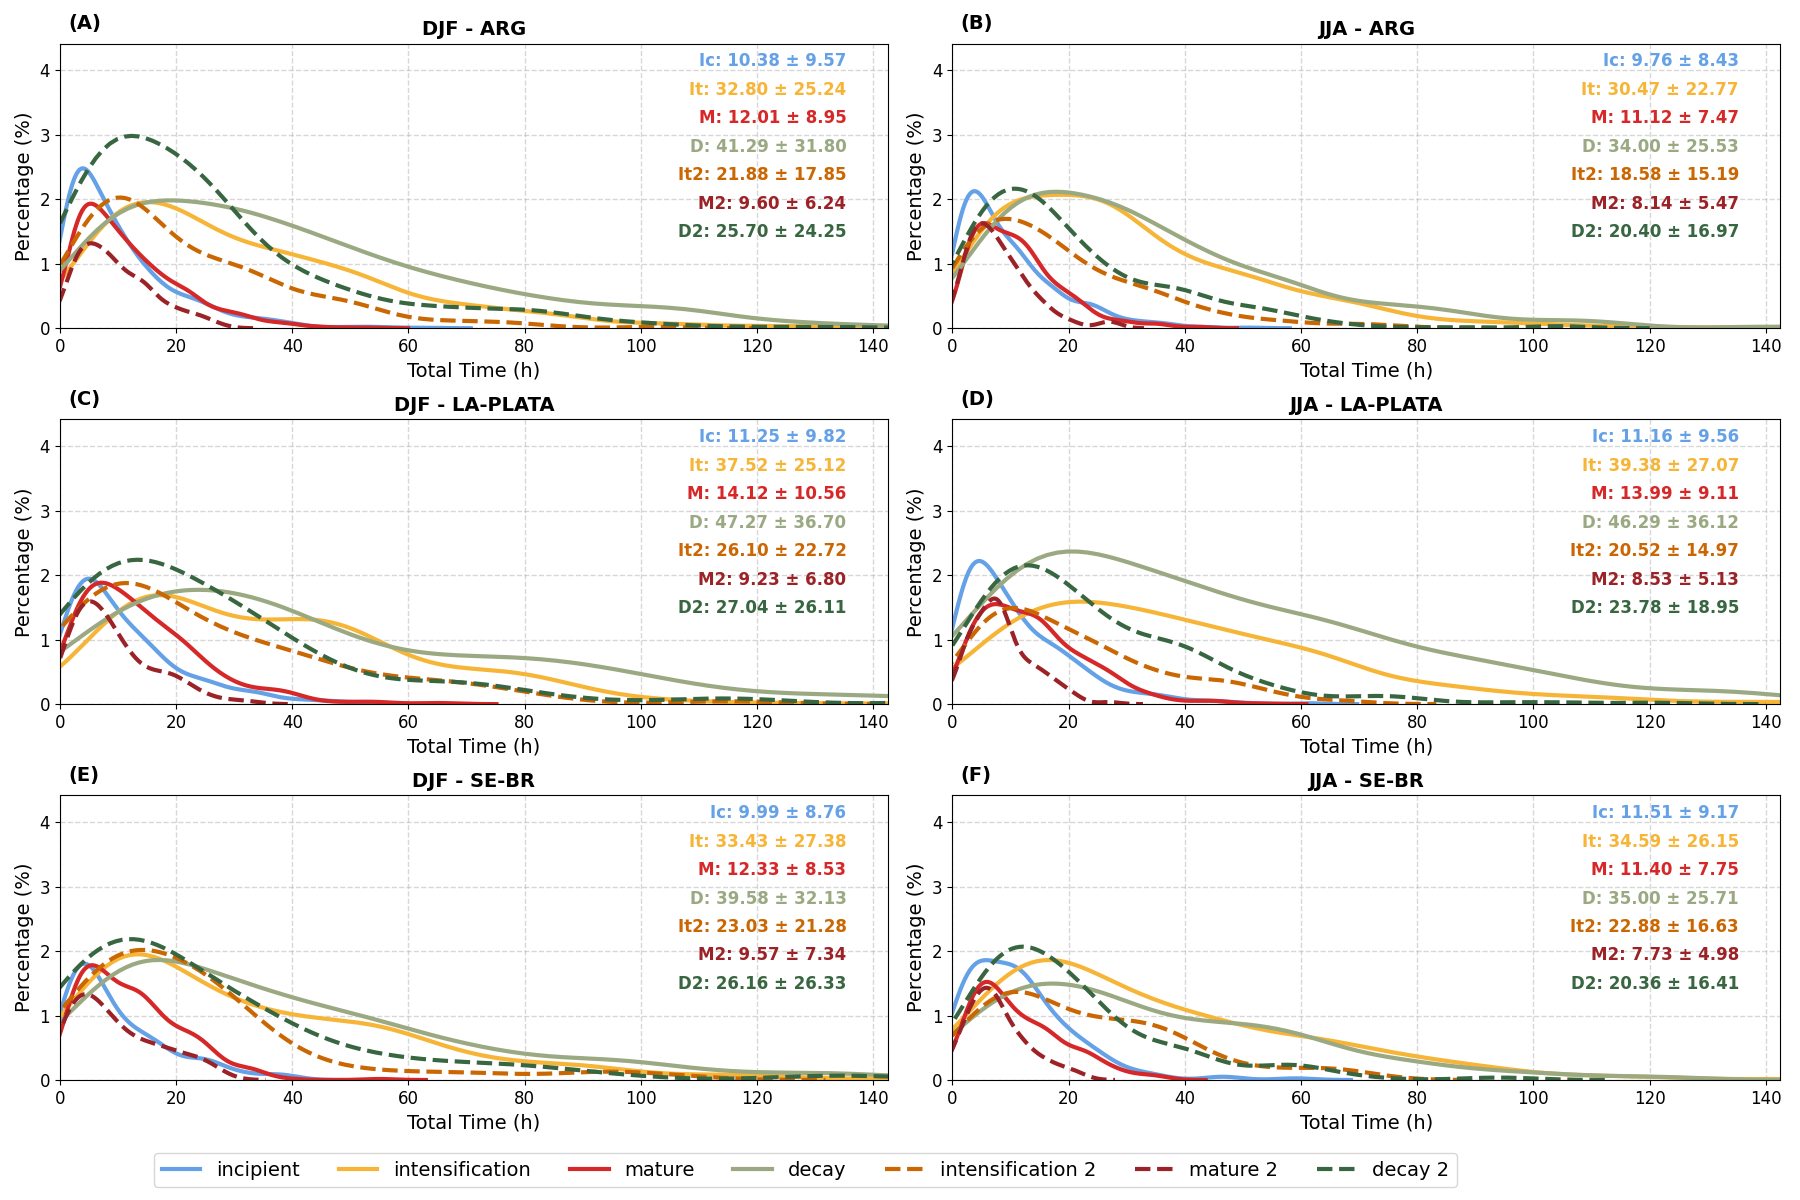
\includegraphics[width=\textwidth]{figs_4/pdf_total_time.png}
\caption[PDF - Total Time]{Probability density functions (PDF) comparing the mean total duration of each cyclone phase, across all regions combined and for each genesis region (ARG, LA-PLATA, SE-BR) for DJF and JJA. Annotations display mean and standard deviation values for each phase.}
\label{fig:pdf_total_time}
\end{figure}

The total traveled distance for each phase is depicted in Figure \ref{fig:pdf_total_distance}, which mirrors the overall behavior observed for total time (Figure \ref{fig:pdf_total_time}). All PDFs are right-skewed, and across all regions and seasons, the incipient, mature, and second mature phases peak approximately between 300 and 400 km, while the other phases present long tail distributions. In the ARG region, there is an overall reduction in traveled distance across all phases from DJF to JJA. Conversely, for LA-PLATA and SE-BR, there is a general increase, reflecting the seasonal behavior for the entire lifecycle's total distance (Figure \ref{fig:pdf_total_time_total}).

\begin{figure}[h!]
\centering
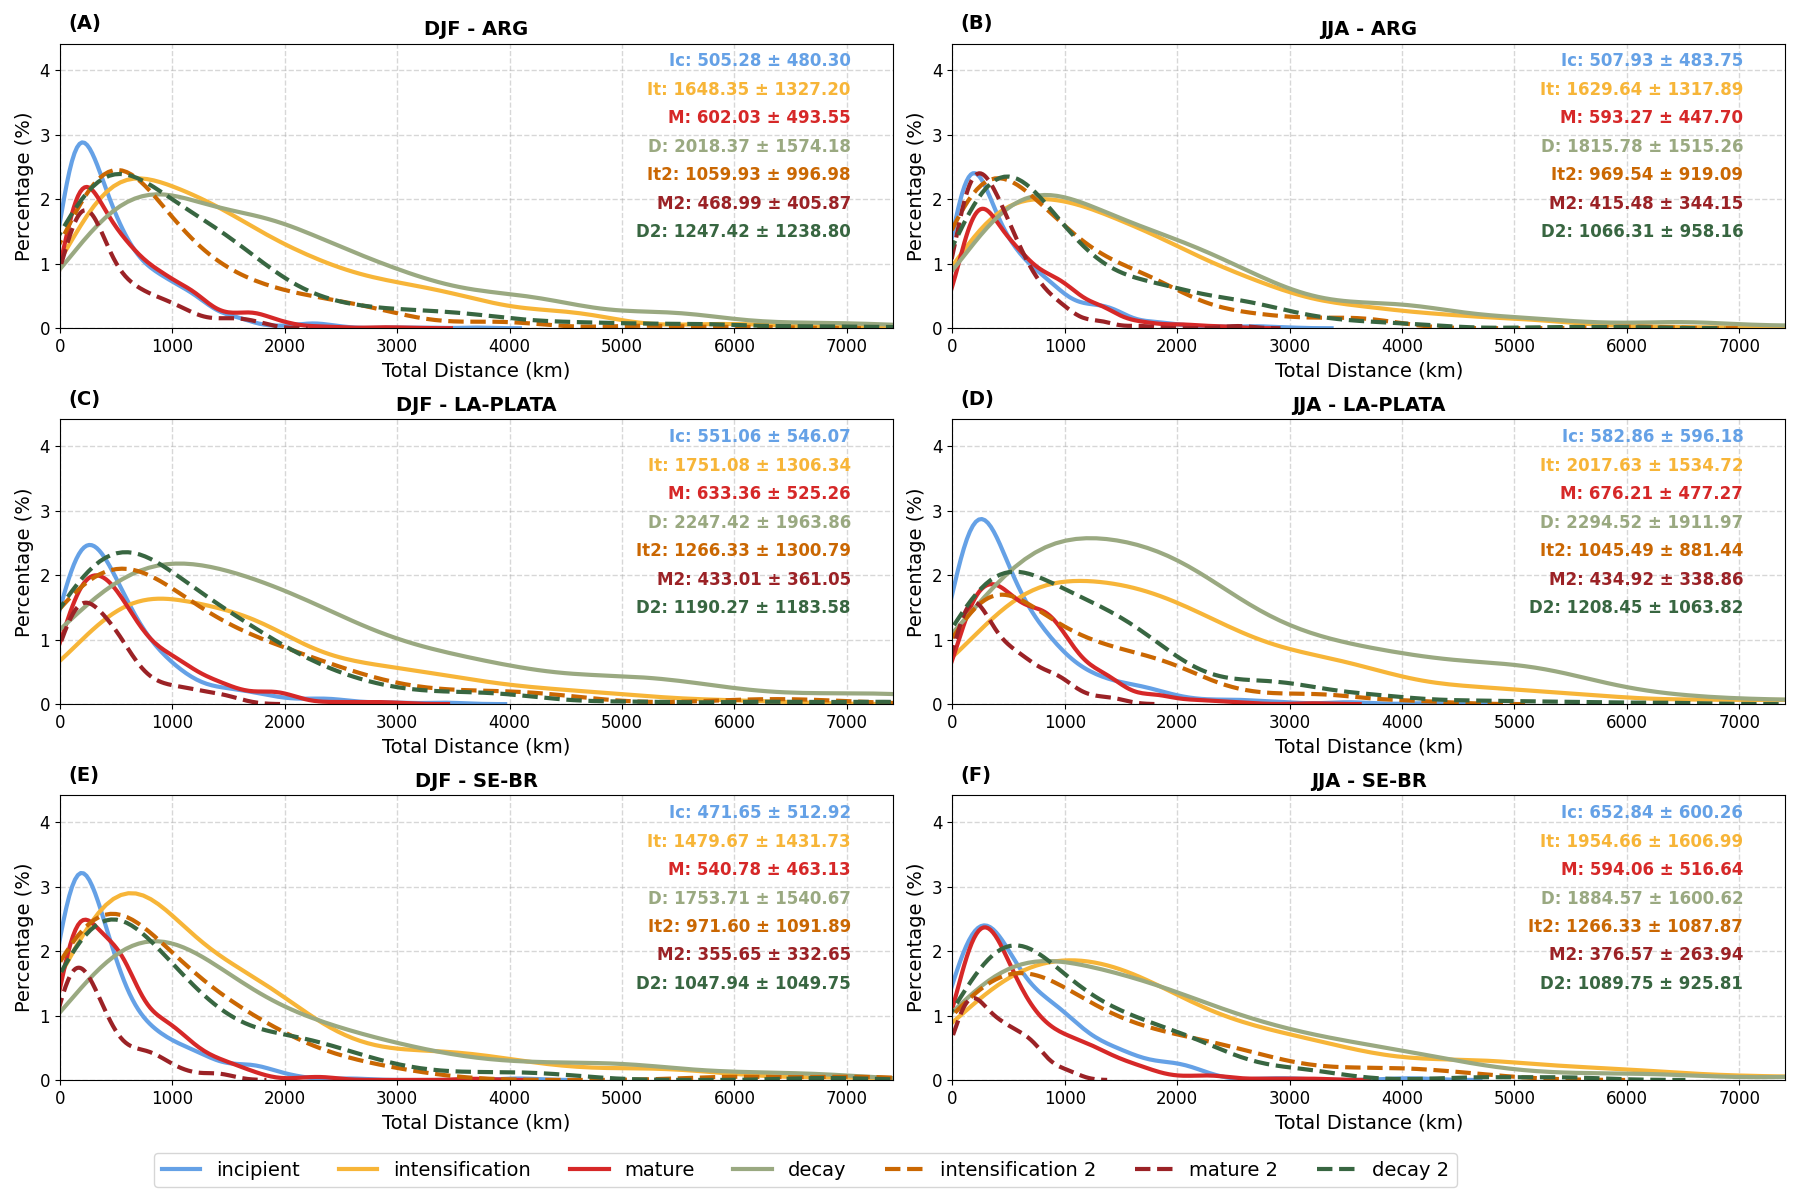
\includegraphics[width=\textwidth]{figs_4/pdf_total_distance.png}
\caption[PDF - Total Distance]{Similar to Figure \ref{fig:pdf_total_time}, but for total traveled distance.}
\label{fig:pdf_total_distance}
\end{figure}

The results for mean speed (Figure \ref{fig:pdf_mean_speed}) aggregate the results for total time and traveled distance. There is less variability across distinct phases for this metric when compared to the total time and distance, with the PDFs for distinct phases, regions, and seasons often presenting a Gaussian-like shape centered between 10 and 15 \(m s^{-1}\). These values align with those found in previous studies \citep{gramcianinov2019properties, gramcianinov2020analysis, hoskins2005new}, although slightly higher, likely due to the constraints adopted in this analysis. Additionally, this study's ability to account for distinct developmental phases provides a foundation for further research into the dynamical mechanisms that could be linked to the systems' varying speeds across different periods. In the ARG region, the largest increases in mean propagation speed from DJF to JJA are found in the secondary development phases, accompanied by increases in standard deviation values, with slightly right-skewed PDFs for these phases. LA-PLATA displays a similar behavior, especially for intensification and mature decay, which shifts their peaks from near \(10 m s^{-1}\) in DJF to near \(15 m s^{-1}\) in JJA. For SE-BR, the major change is in the shape of the PDFs, which change from a Gaussian-like shape in DJF to a more right-skewed shape in JJA. Overall, although the differences are only marginal, the cyclones tend to be faster in the incipient stage and in the intensification stage, being slower at the mature phase, speeding up again in the decay phase. Also, the systems tend to be slower in the second development cycle than in the first one, especially slower at the second mature phase. Therefore, cyclones in the SESA region are slower at their mature phases. The slower propagation speed of cyclones is related to extreme wave occurrence \citep{gramcianinov2023impact} and therefore the positioning of these systems during that phase are of importance for coastal management in the South American Southeastern coast.

\begin{figure}[h!]
\centering
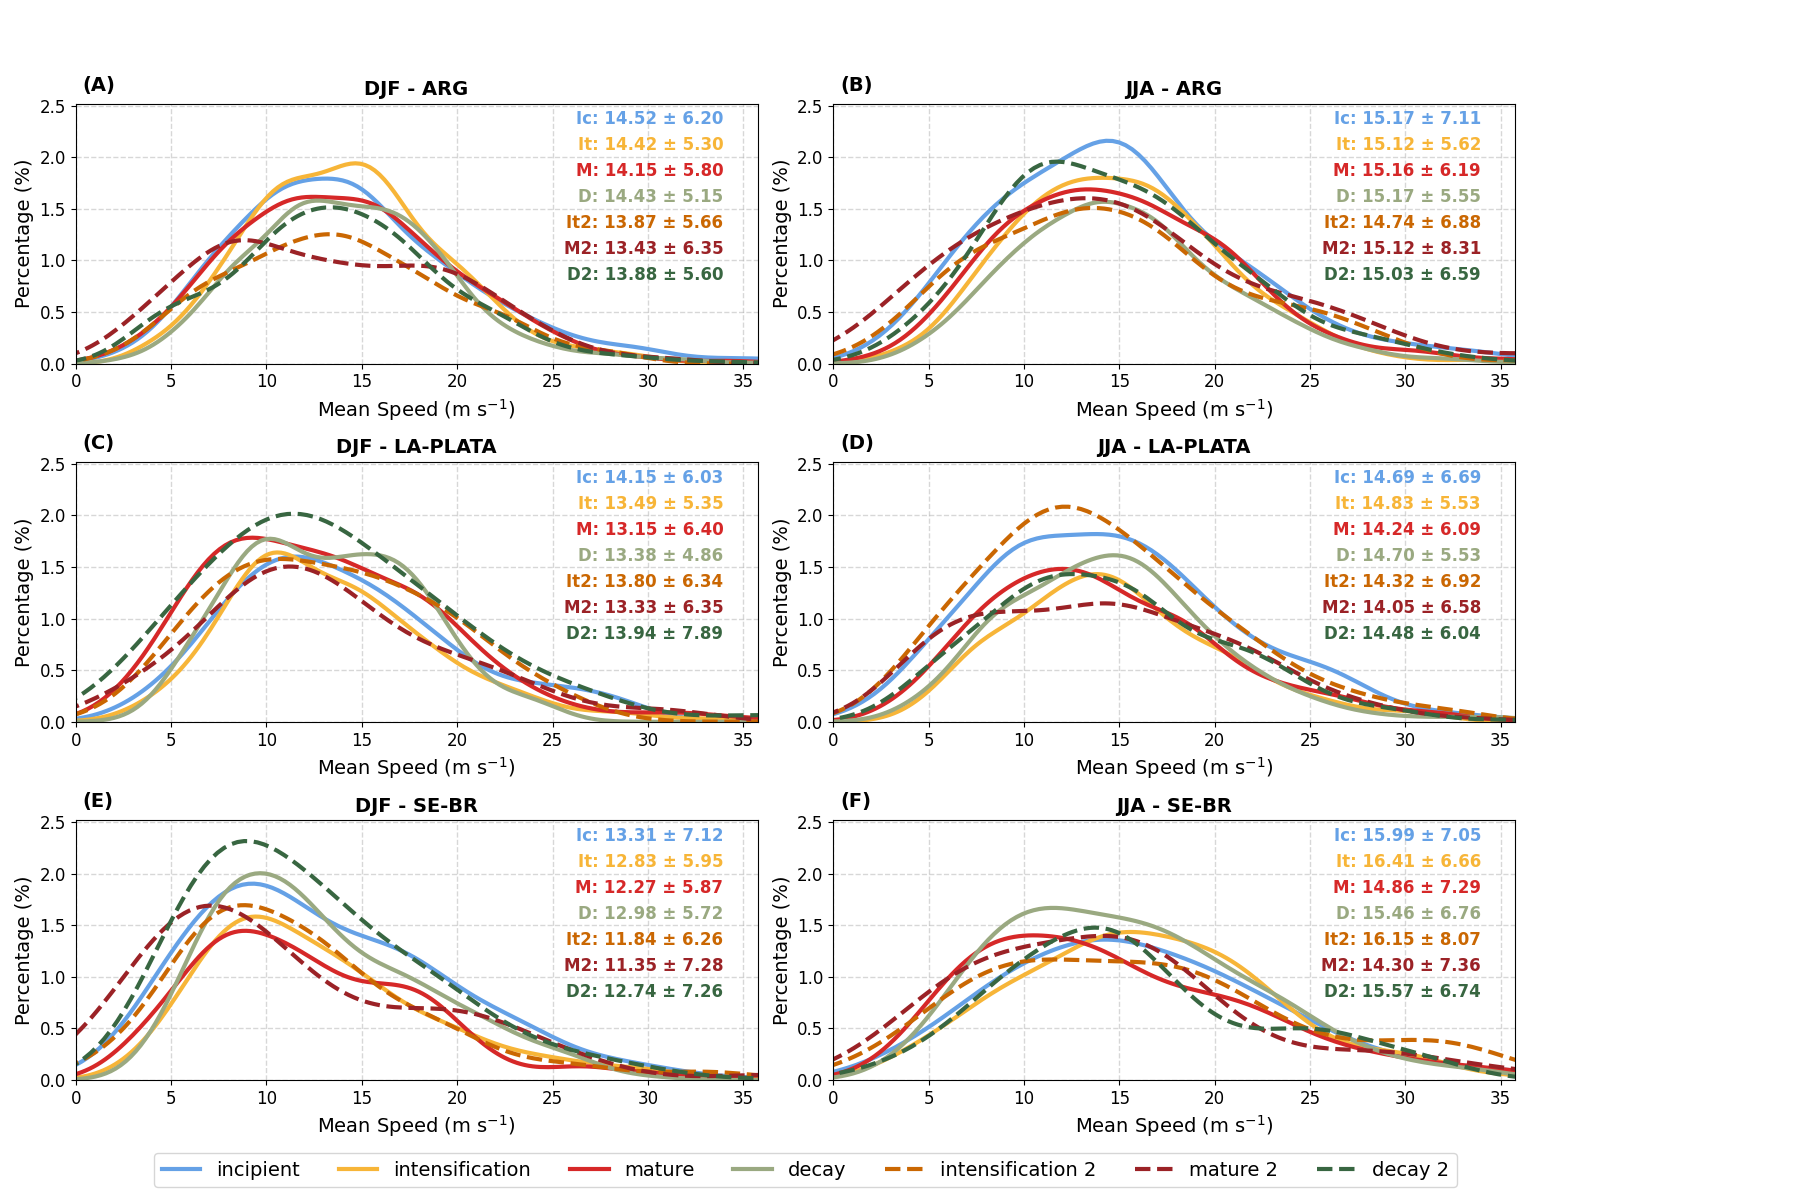
\includegraphics[width=\textwidth]{figs_4/pdf_mean_speed.png}
\caption[PDF - Mean Speed]{Similar to Figure \ref{fig:pdf_total_time}, but for mean propagation speed.}
\label{fig:pdf_mean_speed}
\end{figure}

The PDFs for mean central \(\zeta_{850}\) across various cyclone phases exhibit bimodal and right-skewed distributions, with a general increase in mean vorticity from DJF to JJA (Figure \ref{fig:pdf_mean_vorticity}). This trend reflects the heightened intensity of cyclonic systems during JJA compared to DJF (Figure \ref{fig:pdf_total_time_total}). It is important to note that these vorticity values are derived from the raw output of the TRACK program, and as such, they may include some level of noise that can influence the statistical results. Notably, the mature phase is characteristically the most intense during the first developmental cycle across all regions, demonstrating a wide range of vorticity values and highlighting the variability in peak intensities of mature cyclones. Meanwhile, the second mature phase typically records the highest vorticities among all phases, suggesting a tendency for systems to intensify further during subsequent cycles. In contrast, the incipient phase generally exhibits the lowest mean vorticities, reflecting the nascent stages of cyclone development. However, in the SE-BR region, this phase shows unusually high mean vorticities during JJA, occasionally surpassing other phases, indicating exceptionally conducive conditions for early cyclone formation. The intensification and decay phases generally present similar mean vorticities, aligning with their respective roles in modifying system intensity: intensification increases vorticity from a baseline state, while decay reduces it back towards this baseline. Secondary intensification and decay phases often exhibit higher mean vorticities than their initial counterparts, reflecting the dynamics of re-intensification in the lifecycle, particularly marked by the higher mean values observed during the second mature phase.


\begin{figure}[h!]
\centering
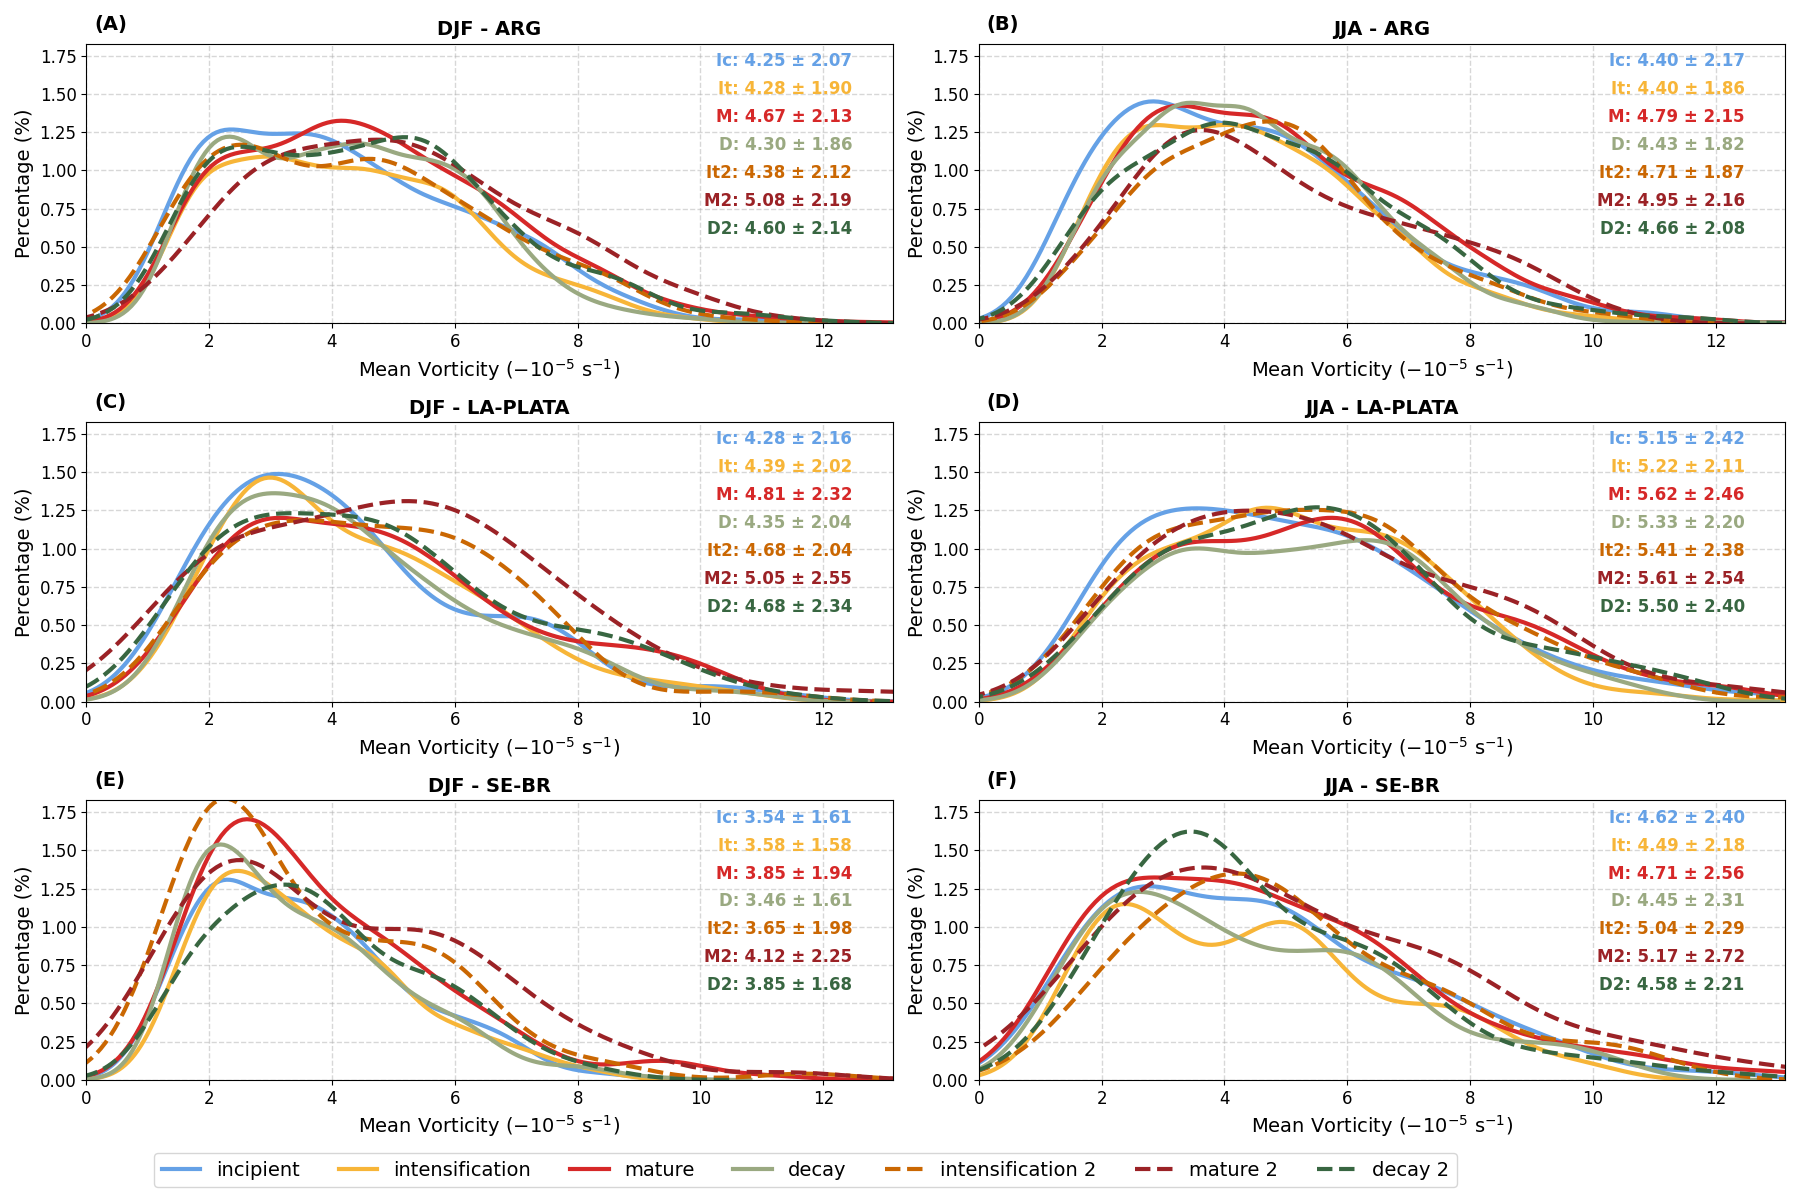
\includegraphics[width=\textwidth]{figs_4/pdf_mean_vorticity.png}
\caption[PDF - Mean Vorticity]{Similar to Figure \ref{fig:pdf_total_time}, but for mean central relative vorticity at cyclone center ($zeta_{850}$).}
\label{fig:pdf_mean_vorticity}
\end{figure}

The results found here for the incipient stage exhibit higher vorticities compared to the initial vorticities reported by \citet{reboita2010south}, \citet{gramcianinov2019properties}, and \citet{gramcianinov2020analysis}. This discrepancy may be attributed to our exclusion criteria, which likely excluded weaker and underdeveloped systems, coupled with the observed tendency for vorticity to increase (becoming more negative) when an incipient stage is followed by an intensification phase (e.g., Figure \ref{fig:representative_life_cycles}a and c), potentially resulting in a bias toward higher values for this phase. Additionally, \citet{sinclair1995climatology}, in their analysis focusing on the first time step, the time step of minimum vorticity, and the last time step, reported higher vorticity values compared to our findings for the incipient, mature, and decay stages. However, these authors omitted the influence of topography by using geostrophic relative vorticity, which justifies the difference in vorticity distribution observed in their study.

There are complexities in interpreting the results for the mean growth rate due to the use of raw vorticity data from the TRACK algorithm, which introduces additional noise to the findings (Figure \ref{fig:pdf_mean_growth_rate}). This metric exhibits considerable variability across different regions, with most PDFs centered around zero yet displaying wide variations, where standard deviations significantly exceed the mean values. The incipient stage often shows the highest or second-highest growth rates, typically skewing more to the right. These observations are consistent with previously reported mean growth rates for cyclogenesis regions by \cite{hoskins2005new} and \cite{gramcianinov2019properties}. A similar pattern is observed in the intensification phase, which alternates with the incipient stage in displaying the greatest growth rates. Despite positive average values, the decay and second decay phases predominantly peak at negative values, reflecting their role in diminishing system vorticity.

\begin{figure}[h!]
\centering
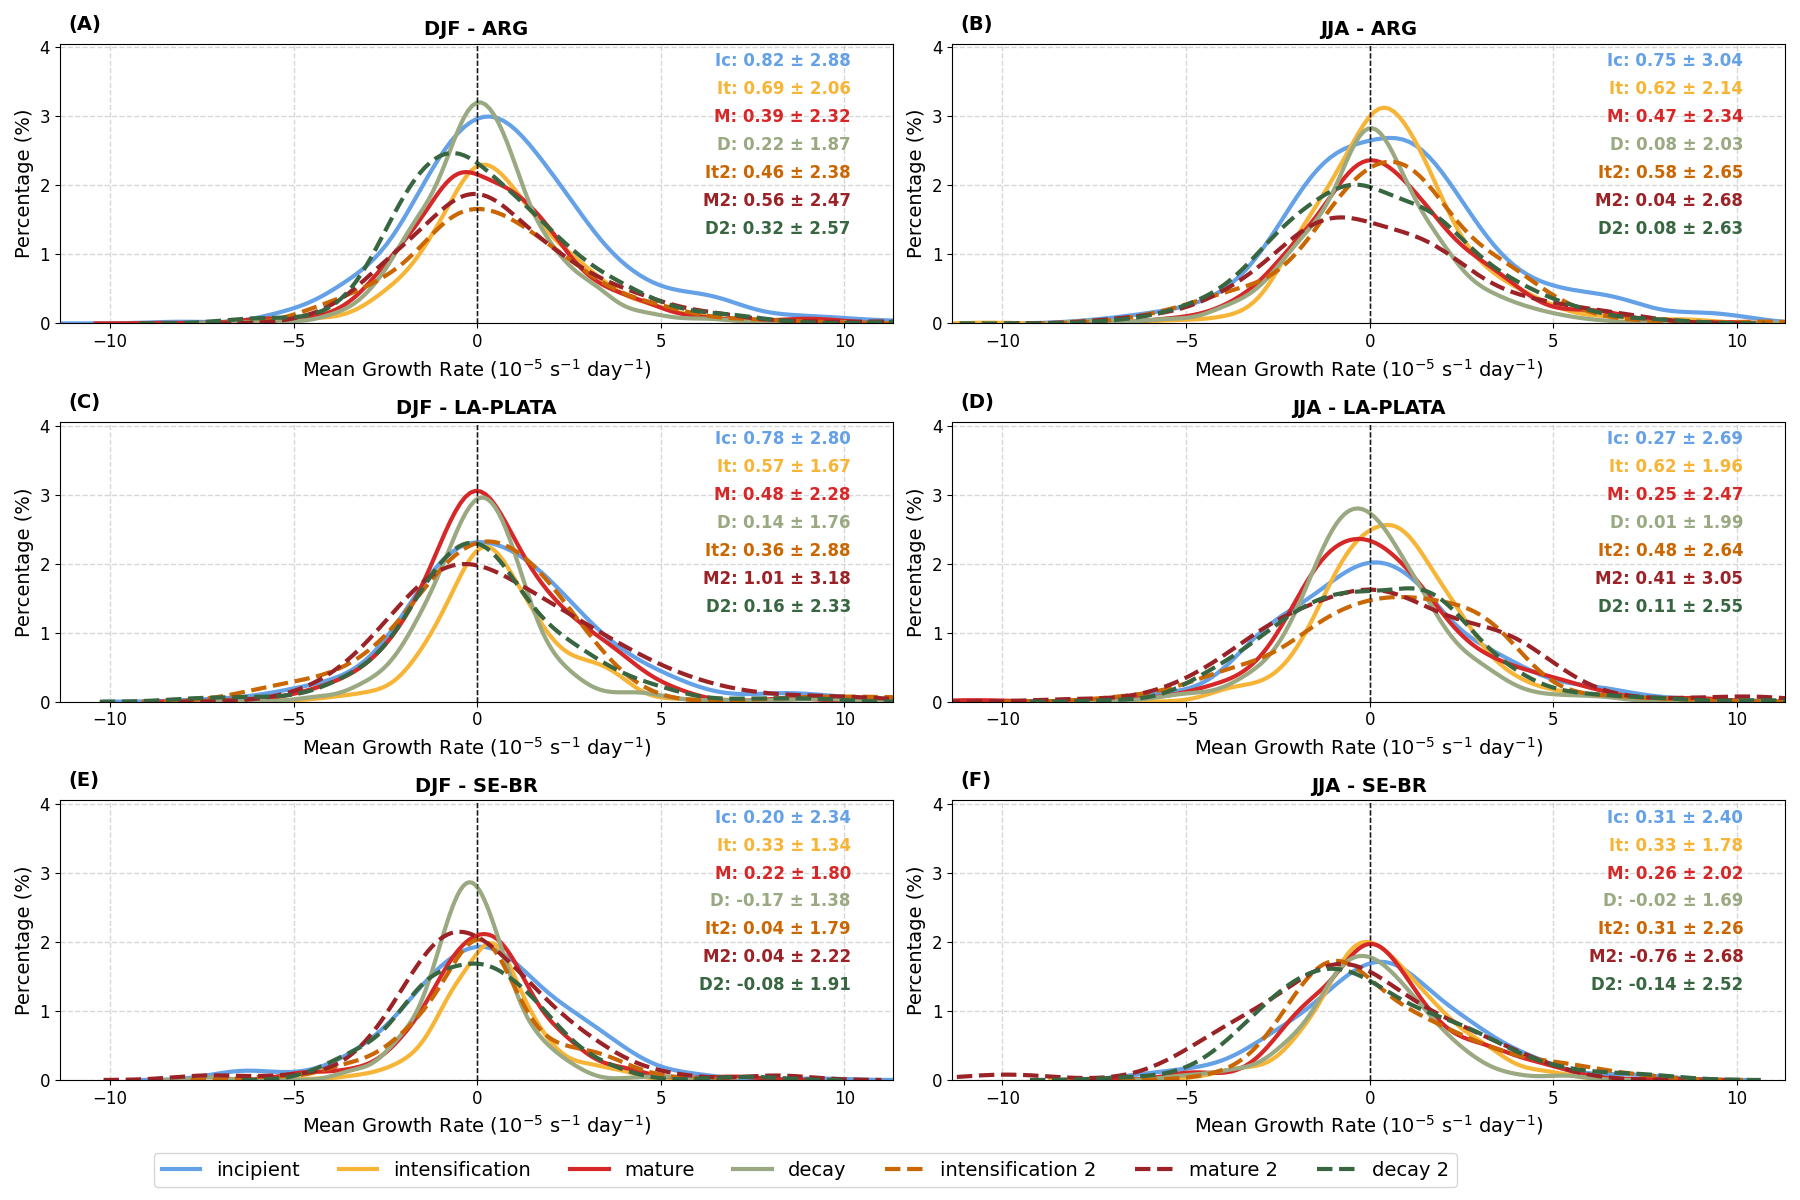
\includegraphics[width=\textwidth]{figs_4/pdf_mean_growth_rate.png}
\caption[PDF - Mean Growth Rate]{Similar to Figure \ref{fig:pdf_total_time}, but for mean growth rate.}
\label{fig:pdf_mean_growth_rate}
\end{figure}


While most regions and seasons show the mature phase peaking at zero — expected due to its position near local vorticity minima — the positive mean suggests that the increase in vorticity preceding the peak is more pronounced than the subsequent decline. This assertion is supported by the lower mean values observed during the decay phase compared to the intensification phase. Moreover, the detection of the mature phase often occurs between the peaks and valleys of vorticity derivatives (Section \ref{sec:cyclophaser_description}), potentially shifting its center of mass toward either the intensification or decay stages, as depicted in Figure \ref{fig:mature_phase}. During JJA in LA-PLATA, the mature phase peaks positively, whereas in SE-BR during DJF, it peaks negatively. Determining whether these shifts are due to greater increases in intensity, displacement of the phase's center of mass, or residual data noise is beyond this study's scope.

\begin{figure}[h!]
\centering
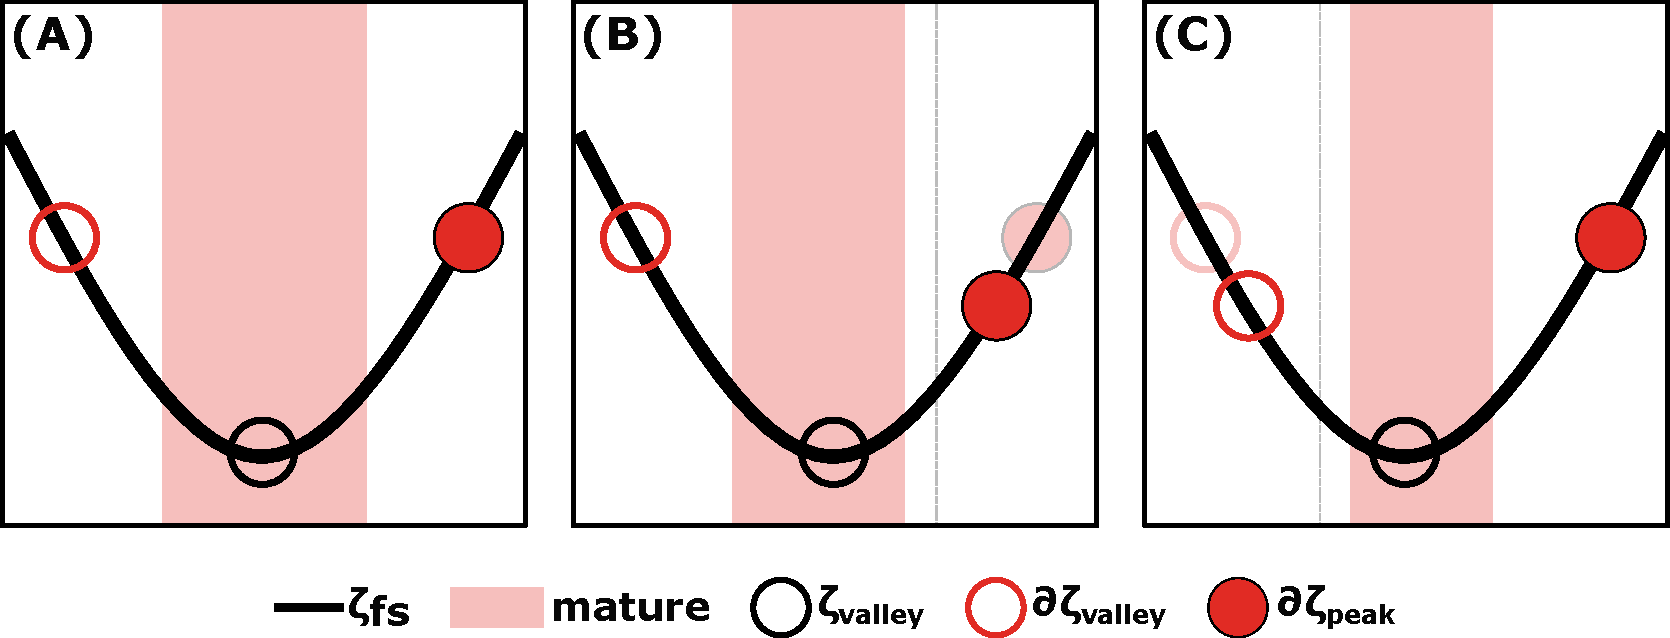
\includegraphics[width=\textwidth]{figs_4/mature_phase.pdf}
\caption[Mature Phase - Center of Mass]{Illustrative example of how the center of mass of the mature phase can be displaced: (A) Symmetrically around the vorticity valley (\(\partial \zeta_{valley}\)) when distances to the first derivative valley (\(\partial \zeta_{valley}\)) and peak (\(\partial \zeta_{peak}\)) are equal. (B) Displacement towards the previous phase when \(\partial \zeta_{peak}\) is closer to \(\zeta_{valley}\). (C) Displacement towards the subsequent phase when \(\partial \zeta_{valley}\) is closer to \(\zeta_{valley}\).}
\label{fig:mature_phase}
\end{figure}

\section{Summary and Concluding Remarks}

\begin{itemize}
    \item This study highlights the importance of SE-BR to cyclone climatology in SESA region: most of previous climatologies indicated SE-BR as a minor genesis region, with weak systems and predominantly active during DJF, but with the constrains adopt here, the underdeveloped systems are remoced and this region presents genesis comparable to LA-PLATA region. Also, its seasonality become less apparent. 
\end{itemize}

